\begin{tikzpicture}
    \node[inner sep=4pt] (photo) at (5,-1.86) {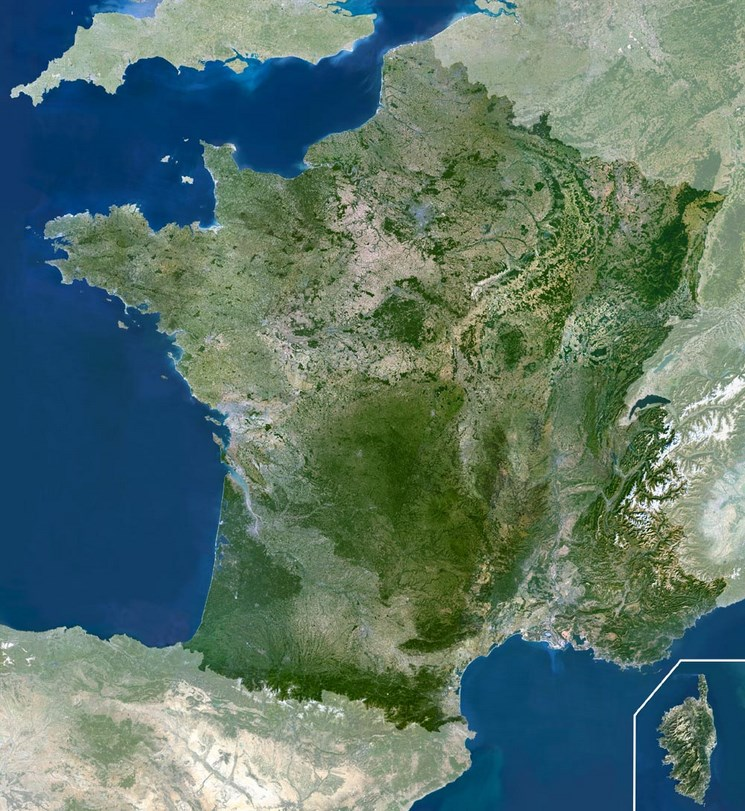
\includegraphics[scale=0.12]{figures/images/france_satellite.jpg}};
    \node[align=center,below] at (photo.south) {Systeme modelise};
    % the local bounding box is to give a name to the pic:
    % http://tex.stackexchange.com/a/241737/32098
    \pic[local bounding box=carte] (carte) at (-5, 0) {france={scale 0.2}};
    \node[align=center,below] at (carte.south) {Modele};
    \draw[->] (carte) -- (photo.west) node[midway,above] {Represente} node[midway,below]{$\mu$};
\end{tikzpicture}

